\documentclass{article}

\usepackage[ngerman]{babel}
\usepackage[T1]{fontenc}
\usepackage[utf8]{inputenc}
\usepackage[a4paper,margin=2.2cm,footskip=0.5cm]{geometry}

\usepackage{mathtools}
\usepackage{amsmath}
\usepackage{amssymb}
\usepackage{ntheorem}
\usepackage{xcolor}

\usepackage{lmodern}
%\usepackage{csquotes}

\usepackage{tikz}
\usetikzlibrary{fit}
%\usetikzlibrary{positioning, fit, calc}

\usepackage{cite}

\usepackage{fancyhdr, lastpage}

\pagestyle{fancy}

\newcommand{\Fpage}{\thepage{}/\pageref{LastPage}}
\newcommand{\Ftitle}{Aufgabe 2 Geburtstag}
\newcommand{\Fauthor}{Nikolas Kilian}

\lhead{\Fauthor}
\rhead{\Ftitle}
\chead{}
\lfoot{}
\rfoot{}
\cfoot{\Fpage}

\setlength{\parskip}{.8em} 
\setlength{\parindent}{0pt}

% Für Algorithmen
\usepackage{algpseudocode}
\usepackage{algorithm}
%\usepackage{pxfonts}

\algnewcommand\algorithmicforeach{\textbf{for each}}
\algdef{S}[FOR]{ForEach}[1]{\algorithmicforeach\ #1\ \algorithmicdo}

%
% Für Quelltext
\usepackage{listings}
\usepackage{xcolor}

\usepackage{url}

\newtheorem{theorem}{Theorem}[section]
\newtheorem{corollary}{Corollary}[theorem]
\newtheorem{lemma}[theorem]{Lemma}

\theoremstyle{nonumberplain}
\theoremheaderfont{\itshape}
\theorembodyfont{\normalfont}
\theoremseparator{.\,—}
\theoremsymbol{}
\newtheorem{proof-wo}{Beweis}
\theoremsymbol{\ensuremath{\color{lightgray}\blacksquare}}
\newtheorem{proof}{Beweis}

%\usepackage{courier}
%\setmonofont{Consolas} %to be used with XeLaTeX or LuaLaTeX
\definecolor{bluekeywords}{rgb}{0,0,1}
\definecolor{greencomments}{rgb}{0,0.5,0}
\definecolor{redstrings}{rgb}{0.64,0.08,0.08}
\definecolor{xmlcomments}{rgb}{0.5,0.5,0.5}
\definecolor{types}{rgb}{0.17,0.57,0.68}
\definecolor{turqoisetypes}{rgb}{0.01,0.60,0.3}
\definecolor{background}{rgb}{0.95,0.95,0.95}
%\definecolor{background}{rgb}{.97,.97,.97}

\newcommand{\codesize}{\small}

\lstdefinelanguage{CSharp}{ % Better C# highlighting
language=[Sharp]C,
frame=lrbt,
%language=general,
backgroundcolor=\color{background},
captionpos=b,
numbers=left,
numberstyle=\tiny,
showspaces=false,
showtabs=false,
breaklines=true,
showstringspaces=false,
breakatwhitespace=true,
escapeinside={(*@}{@*)},
commentstyle=\color{greencomments},
morekeywords={partial, var, get, set, from, select, package, deref},
%
emph=[0]{T,U,V,TToken},
emphstyle=[0]{\color{types}},
%
emph=[1]{NotSupportedException,List,HashSet,Map,Street,Vector2Int,DirectedVector2Int,StreetParser},
emphstyle=[1]{\color{turqoisetypes}},
%
otherkeywords={=>,<,>},
emph=[2]{=>,<,>},
emphstyle=[2]{\bfseries},
%
emph=[3]{ParserResult},
emph=[3]{\color{turqoisetypes}\bfseries},
%
keywordstyle=\color{bluekeywords},
stringstyle=\color{redstrings},
basicstyle=\codesize\ttfamily,
literate=%
    {Ö}{{\"O}}1
    {Ä}{{\"A}}1
    {Ü}{{\"U}}1
    {ß}{{\ss}}1
    {ü}{{\"u}}1
    {ä}{{\"a}}1
    {ö}{{\"o}}1
    {~}{{\textasciitilde}}1
}

\lstMakeShortInline[
  language=CSharp,
  columns=fixed,]~

  \lstnewenvironment{lstcs}[1][]
  {\lstset{
      language=CSharp,
      breaklines=true,
      columns=fullflexible,
      caption={#1}
  }}
{}

\usepackage{hyperref}
\usepackage{cleveref}

\begin{document}
    
\section{Lösungsidee}

Die Lösungsidee besteht darin, den Dijkstra Algorithmus derart umzugestalten, dass er den Weg mit der geringsten Zahl an Abbiegungen statt der geringsten Länge sucht.
Zuerst wird der kürzeste Weg berechnet, woraufhin dessen Länge und die Anzahl der darin enthaltenen Abbiegungen bestimmt wird. Daraufhin beginnt die Ermittlung des endgültigen Weges.

Grundlegend verläuft dieser Prozess wie der normale Dijkstra Algorithmus, jedoch mit ein paar kleinen Unterschieden:
Der erste Unterschied besteht darin, dass der Algorithmus alle Wege mit einer Länge größer der Länge des kürzesten Wegs plus die erlaubte Extrastrecke (also +15\% oder +30\%) eliminiert.
Der Hauptunterschied besteht jedoch darin, dass Dijkstra hierbei nicht nach Länge, sondern nach Anzahl an Abbiegungen optimiert.

\subsection{Modifizierter Dijkstra im Detail}

Um Dijkstra im Hinblick auf die minimale Anzahl an Abbiegungen umzudefinieren, könnte die zugrunde liegende Kostenfunktion anstelle der Länge des Graphen die Existenz von Abbiegungen betrachten, entweder mit einer '1' für eine Abbiegung oder einer '0' für eine Gerade. 
Dabei fällt auf, dass zur Berechnung der Kosten für eine Kante auch die im Weg vorangehende Kante betrachtet werden muss.
Dies bedeutet aber, dass Dijkstra nicht in seiner ursprünglichen Form verwendet werden kann. Es könnte ansonsten der Fall auftreten, dass Knoten des Graphen von einem anderen Weg aus erneut besucht würden, was die Kosten der Kanten verändern würde, die mit dem Knoten verbunden sind.

\begin{center}
\begin{tikzpicture}
    \node (A) at (1, 1){A};
    \coordinate (AB) at (6,1);
    \node (D) at (11, 1){D};
    
    \node (C) at (1, 5){C};
    \coordinate (CD) at (6, 5) {};
    \node (B) at (11, 5){B};
    
    \coordinate (ABCD) at (6, 3);
    \node [draw,dashed,inner sep=10pt, circle,yscale=.7, fit={(ABCD)}] {};
    
    \draw[-, thick] (A) to node[midway, sloped, above] {}  (ABCD);
    \draw[-, thick] (ABCD) to node[midway, sloped, above] {}  (D);
    \draw[-, thick] (C) to node[midway, sloped, above] {}  (ABCD);
    \draw[-, thick] (ABCD) to node[midway, sloped, above] {}  (B);
\end{tikzpicture}
\end{center}

Um dieses Problem zu umgehen, wird der Graph verändert: Zwar werden
Kreuzungen innerhalb des Graphen immer noch als Knoten dargestellt, jedoch gibt es für jede Kreuzung mehrere Knoten, nämlich jeweils einen für jede geradlinige Straße, die in der Kreuzung vorhanden ist.
Alle Knoten einer Kreuzung sind dabei verbunden durch Kanten mit Kosten von 1.

\begin{center}
\begin{tikzpicture}
    \node (A) at (1, 1) {A};
    \coordinate (AB) at (6,2);
    \node (B) at (11, 1) {B};
    
    \node (C) at (1, 5){C};
    \coordinate (CD) at (6, 4) {};
    \node (D) at (11, 5){D};
    
    \node [rotate=90][draw,dashed,inner sep=5pt, circle,yscale=.6, fit={(AB) (CD)}] {};
    
    %\draw[-, thick] (A) to node[midway, sloped, above] {A--Cross}  (AB);
    \draw[-, thick] (A) to node[midway, sloped, below] {0}  (AB);
    %\draw[-, thick] (AB) to node[midway, sloped, above] {Cross--B}  (B);
    \draw[-, thick] (AB) to node[midway, sloped, below] {0}  (B);
    %\draw[-, thick] (C) to node[midway, sloped, above] {C--Cross}  (CD);
    \draw[-, thick] (C) to node[midway, sloped, below] {0}  (CD);
    %\draw[-, thick] (CD) to node[midway, sloped, above] {Cross--D}  (D);
    \draw[-, thick] (CD) to node[midway, sloped, below] {0}  (D);
    
    \draw[-, thick] (AB) to node[midway, sloped, above] {Extra} (CD);
    \draw[-, thick] (AB) to node[midway, sloped, below] {1} (CD);
\end{tikzpicture}
\end{center}

Die Priority-Queue des Dijkstra-Algorithmus ist hierbei primär nach Anzahl an Abbiegungen und sekundär nach Länge sortiert.

Der endgültige Algorithmus geht dann wie folgt vor:

\begin{enumerate}
    \item Initialisiere eine leere Priority-Queue von Wegen.
    \item Füge den Startpunkt als Weg ohne Länge und Abbiegungen hinzu.
    \item Nehme den obersten Weg aus der Priority-Queue (mit den wenigsten Abbiegungen und kürzester Länge).
    \item Ermittle alle Wege, die aus diesem entspringen und noch nicht vorher betrachtet wurden.
    \item Speichere alle Wege zu einer Kreuzung (inklusive Richtung, in der diese befahren wird), die besser als die bisherigen Wege sind und füge diese der Priority-Queue hinzu. Dabei werden eingefügte Elemente primär nach Abbiegung und sekundär nach Weglänge sortiert werden.
    \item Wiederhole 3-5, bis das Ziel an der Spitze der Priority-Queue ist.
\end{enumerate}

\section{Umsetzung}

Der Algorithmus wurde in C\# 8.0 mit .NET Core 3.1 implementiert.
Es wurde als Library OptimizedPriorityQueue\footnote{https://github.com/BlueRaja/High-Speed-Priority-Queue-for-C-Sharp} verwendet. Diese implementiert eine Priority Queue, die in Dijkstra verwendet wird.
Der Code ist in zwei Projekte geteilt;
~Afg3Abbiegen.GUI~ und ~Afg3Abbiegen~.

~Afg3Abbiegen.GUI~ kümmert sich um das User-Interface und ruft ~Afg3Abbiegen~ auf, das den eigentlichen Algorithmus enthält.
~Afg3Abbiegen~ definiert einige Typen:

\begin{description}
    \item[Vector2Int] stellt einen zweidimensionalen Vektor mit Integerkomponenten dar.
    \item[DirectedVector2Int] stellt die Kombination einer ~Vector2Int~ Position und einer genormten Richtung dar.
    \item[Street] definiert eine Straße zwischen zwei ~Vector2Int~ Endpunkten.
    \item[MapParser] ist zuständig für das Einlesen der Beispieldateien.
    \item[EnumerableExtensions] definiert eine Erweiterungsmethode für ~IEnumerable<Vector2Int>~, die die Anzahl an Abbiegung zählt und eine, die die .
    \item[Map] stellt eine Ansammlung aus Straßen mit Start und Ende dar und enthält den Hauptalgorithmus. 
\end{description}

~Map~ definiert dabei zwei Hauptmethoden
~ShortestPath~ und ~BilalsPath~.
~ShortestPath~ ermittlet via Dijkstra den kürzesten Weg zwischen Start und Ende.
~BilalsPath~ ermittelt via dem obigen Algorithmus den in der Aufgabenstellung beschriebenen Weg.

Zur Verwendung des Programms gibt es ein GUI.
Zuerst muss mit ``Load Map'' eine der Beispieldateien geladen werden, danach kann unter ``Factor by which the path may be longer'' der Faktor, um den Bilals Weg länger als der kürzeste Weg sein darf eingegeben werden, also \(1.15\) für \(+15\%\) oder \(1.30\) für \(+30\%\).
Der kürzeste Weg ist in rot dargestellt, Bilals Weg ist grün dargestellt.
Der Startpunkt ist grün markiert, das Ziel rot.

\section{Beispiele}

\newcommand{\incgra}[1]{
    \begin{center}
        \makebox[\textwidth]{\includegraphics[width=\paperwidth]{#1}}
    \end{center}
}

\subsection{}

\begin{center}
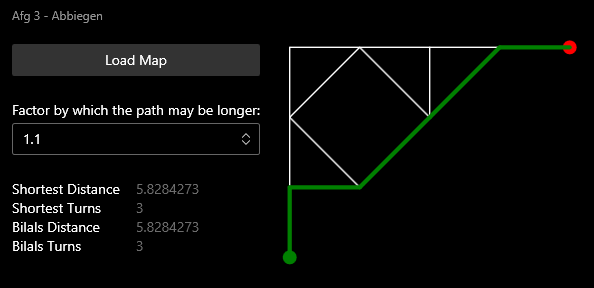
\includegraphics{examples/0_10.png}
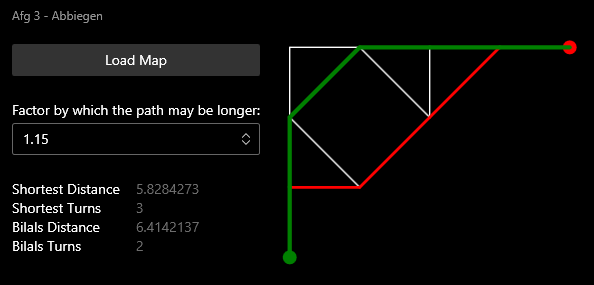
\includegraphics{examples/0_15.png}
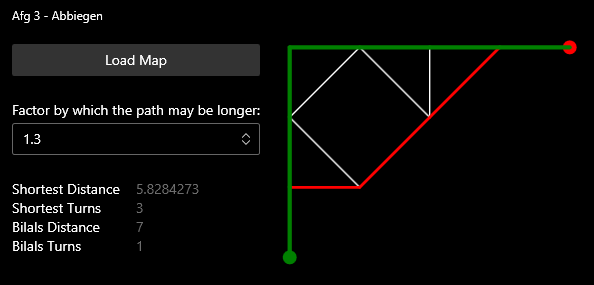
\includegraphics{examples/0_30.png}
\end{center}

\subsection{}

\begin{center}
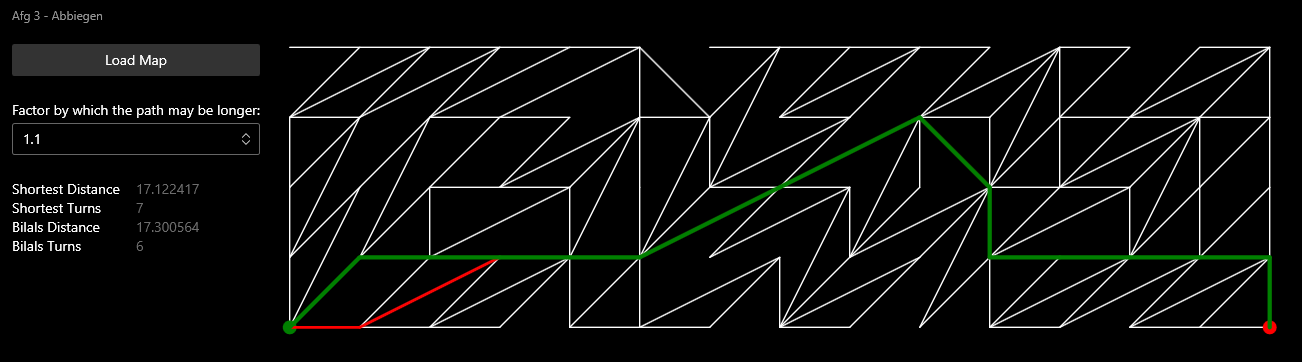
\includegraphics{examples/1_10.png}
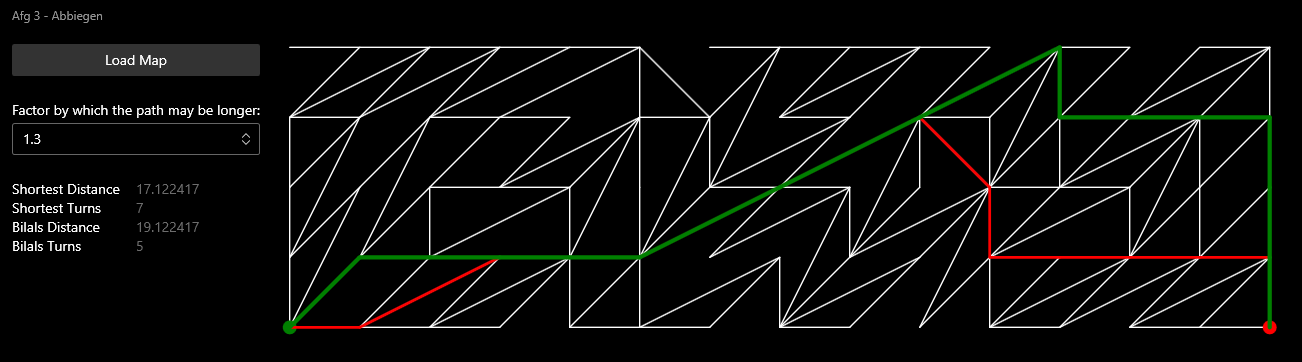
\includegraphics{examples/1_30.png}
\end{center}

\subsection{}

\begin{center}
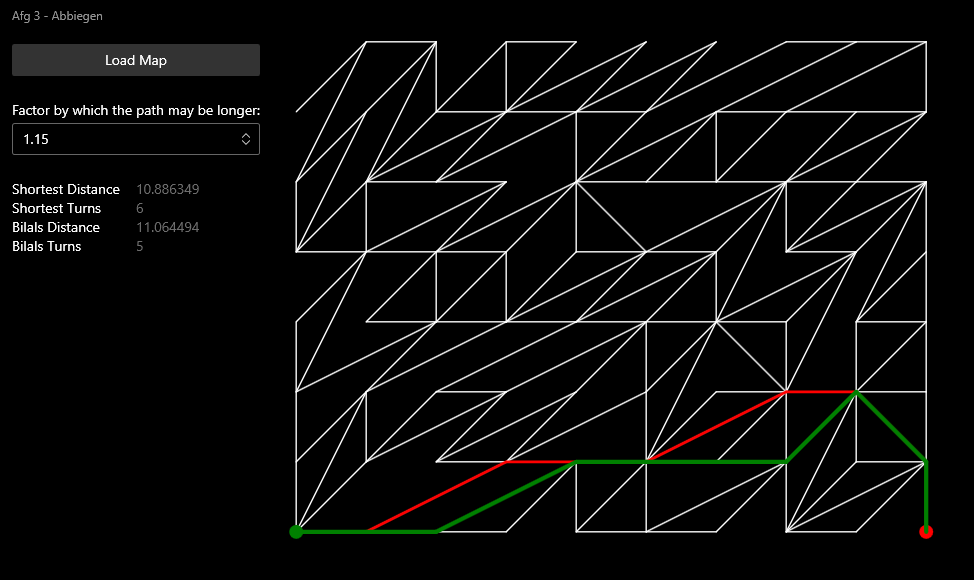
\includegraphics{examples/2_15.png}
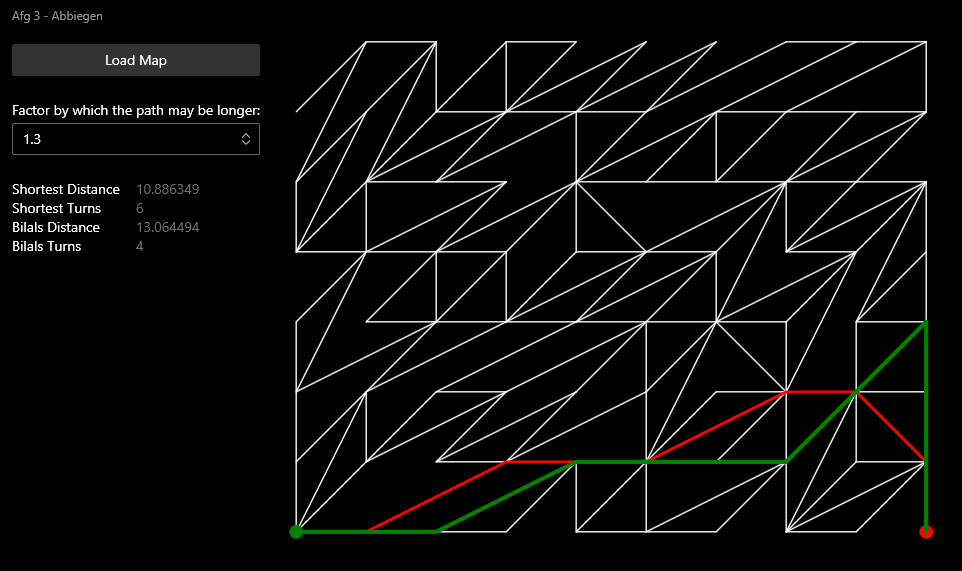
\includegraphics{examples/2_30.png}
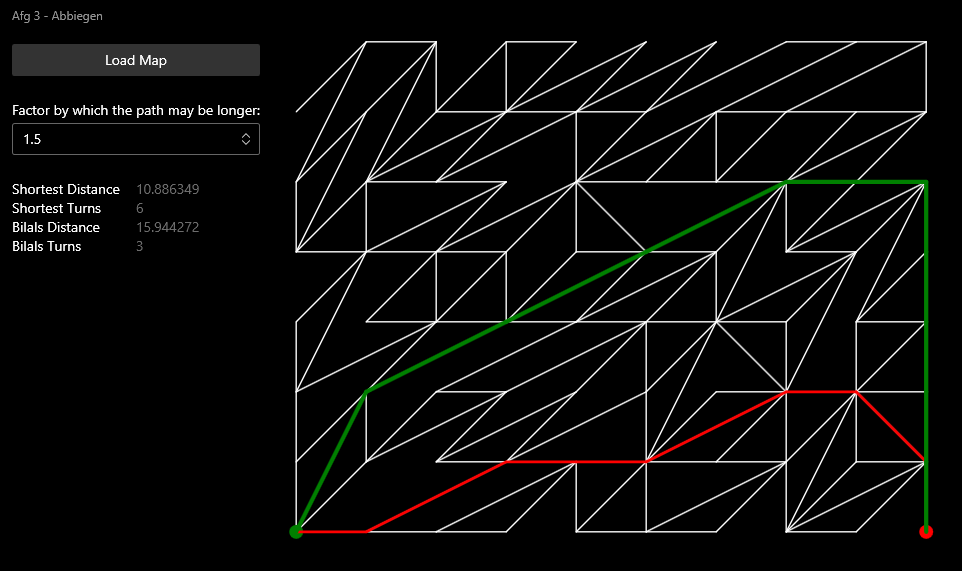
\includegraphics{examples/2_50.png}
\end{center}

\subsection{}

\begin{center}
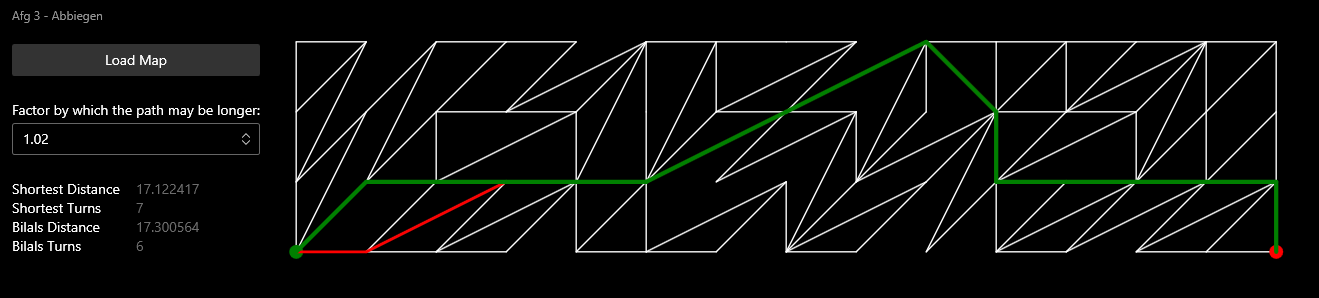
\includegraphics{examples/3_02.png}
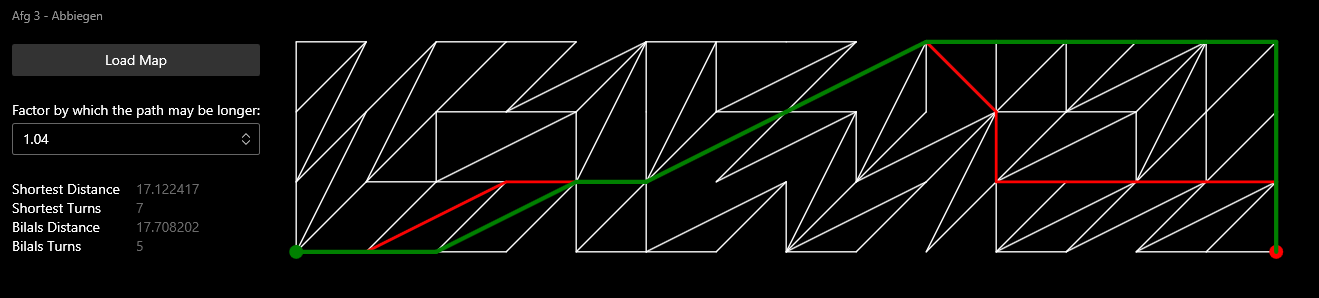
\includegraphics{examples/3_04.png}
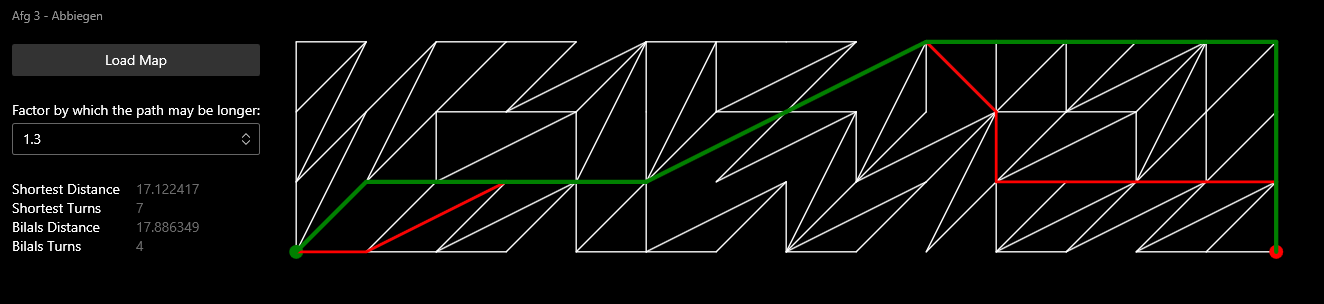
\includegraphics{examples/3_30.png}
\end{center}

\section{Code}

\begin{lstcs}[]
/// <summary>
/// Represents a street between two points.
/// </summary>
public readonly struct Street : IEquatable<Street>
{
    /// <summary>
    /// The start of the street.
    /// </summary>
    public readonly Vector2Int Start;

    /// <summary>
    /// The end of the street.
    /// </summary>
    public readonly Vector2Int End;

    public Street(Vector2Int start, Vector2Int end)
    {
        Start = start;
        End = end;
    }

    /// <summary>
    /// Gets a new with <see cref="Start"/> being equal to <see cref="End"/> of <c>this</c> and vice versa.
    /// </summary>
    public readonly Street Flipped => new Street(End, Start);

    /// <summary>
    /// Returns the path from start to end.
    /// </summary>
    public readonly Vector2Int Path => End - Start;

    // -- Boilerplate ausgelassen --
}
\end{lstcs}

\begin{lstcs}[]
/// <summary>
/// Represents a <see cref="Vector2Int"/> with a direction.
/// </summary>
public readonly struct DirectedVector2Int : IEquatable<DirectedVector2Int>
{
    /// <summary>
    /// The position.
    /// </summary>
    public readonly Vector2Int Position;

    /// <summary>
    /// The direction.
    /// </summary>
    public readonly Vector2Int Direction;

    // -- Boilerplate ausgelassen --
}
\end{lstcs}

\begin{lstcs}[]
/// <summary>
/// Represents a map.
/// </summary>
public class Map
{
    /// <summary>
    /// The list of all streets.
    /// </summary>
    public List<Street> Streets { get; }

    /// <summary>
    /// The position of the starting point.
    /// </summary>
    public Vector2Int Start { get; }

    /// <summary>
    /// The position of the target.
    /// </summary>
    public Vector2Int End { get; }

    /// <summary>
    /// Maps the positions of intersections to all intersections directly reachable from it.
    /// The reachable intersections are specified by their position (Target), the direction they're in (Direction) and their distance form the other intersection (Distance).
    /// </summary>
    public Dictionary<Vector2Int, List<(Vector2Int Target, Vector2Int Direction, float Distance)>> ReachableFromIntersection { get; }

    /// <summary>
    /// Positions of all intersections.
    /// </summary>
    public HashSet<Vector2Int> Intersections { get; }

    /// <summary>
    /// The smallest x and y coordinates of any intersection.
    /// </summary>
    public Vector2Int Min { get; }

    /// <summary>
    /// The largest x and y coordinates of any intersection.
    /// </summary>
    public Vector2Int Max { get; }

    /// <summary>
    /// The difference between the largest and smallest x and y coordinates of any intersection.
    /// </summary>
    public Vector2Int Size { get; }

    public static Map FromText(string[] text)
    {
        if (!MapParser.TryParse(text, out var start, out var end, out var streets)) throw new FormatException();

        return new Map(streets, start, end);
    }

    public Map(List<Street> streets, Vector2Int start, Vector2Int end)
    {
        Streets = streets;
        Start = start;
        End = end;
        ReachableFromIntersection = new Dictionary<Vector2Int, List<(Vector2Int Target, Vector2Int Direction, float Distance)>>();
        Intersections = new HashSet<Vector2Int>();

        // Adds a street to the intersection at its starting point
        void registerStreet(Street street)
        {
            // Get the existing list or add a new one for key street.Start
            var reachableIntersections = ReachableFromIntersection.GetOrCreateValue(street.Start);

            reachableIntersections.Add((street.End, street.Path.Direction, street.Path.Length));

            Intersections.Add(street.Start);
        }

        // Add all streets to all intersections
        foreach (var street in streets)
        {
            registerStreet(street);
            // Both ends are intersections => flip to register the other
            registerStreet(street.Flipped);
        }

        // Save these for the UI
        Min = new Vector2Int(
            Streets.Min(x => Math.Min(x.Start.X, x.End.X)),
            Streets.Min(x => Math.Min(x.Start.Y, x.End.Y)));
        Max = new Vector2Int(
            Streets.Max(x => Math.Max(x.Start.X, x.End.X)),
            Streets.Max(x => Math.Max(x.Start.Y, x.End.Y)));
        Size = Max - Min;
    }

    /// <summary>
    /// Gets the shortest path as computed by dijkstras.
    /// </summary>
    /// <param name="fullDistance">The length of the computed path.</param>
    /// <returns>The path from starting point to ending point, including those points.</returns>
    public IEnumerable<Vector2Int> ShortestPath(out float fullDistance)
    {
        // The position a point is reached from on the shortest currently known path leading to it.
        var paths = new Dictionary<Vector2Int, Vector2Int>();
        // The distance of the shortest currently known path to a given point.
        var distances = new Dictionary<Vector2Int, float>();

        var priorityQueue = new SimplePriorityQueue<Vector2Int, float>();

        foreach (var intersection in Intersections)
        {
            var distance = intersection == Start ? 0 : float.PositiveInfinity;
            priorityQueue.Enqueue(intersection, distance);
            distances[intersection] = distance;
        }

        while (true) // Loop forever. Stop condition is handeled by a break.
        {
            var head = priorityQueue.Dequeue();
            var headDistance = distances[head];

            // End is at the top of the priority queue => the path to End is the shortest unvisited path => finished, break
            if (head == End)
            {
                fullDistance = headDistance;
                break;
            }

            var reachableStreets = ReachableFromIntersection[head];

            foreach (var (target, _, distance) in reachableStreets)
            {
                var oldDistance = distances[target];

                var newDistance = headDistance + distance;

                if (newDistance > oldDistance) continue;

                // Update the priority only if the key already exists. Otherwise add it again.
                if (!priorityQueue.TryUpdatePriority(target, newDistance)) priorityQueue.Enqueue(target, newDistance);

                paths[target] = head;
                distances[target] = newDistance;
            }
        }

        var path = new List<Vector2Int>();
        for (var current = End; current != Start; current = paths[current]) path.Add(current);
        path.Add(Start);
        // Reverse such that Start is actually at the start and End at the end.
        path.Reverse();

        return path;
    }

    /// <summary>
    /// For use in <see cref="BilalsPath(int, float, out int, out float)"/>.
    /// </summary>
    protected class Path : IComparable<Path>, IEquatable<Path>
    {
        public readonly int Turns;
        public readonly float Distance;
        public readonly Vector2Int End;
        public readonly Vector2Int Direction;
        public readonly Path? Previous;

        public Path(int turns, float distance, Vector2Int end, Vector2Int direction, Path previous)
        {
            Turns = turns;
            Distance = distance;
            End = end;
            Direction = direction;
            Previous = previous;
        }

        public Path(Vector2Int end)
        {
            Turns = 0;
            Distance = 0;
            End = end;
            Direction = default;
            Previous = null;
        }

        /// <summary>
        /// Returns a new <see cref="Path"/> instance with <see cref="Previous"/> set to this and <see cref="End"/> set to <paramref name="next"/>.
        /// </summary>
        /// <param name="next">The <see cref="End"/> of the new <see cref="Path"/> instance.</param>
        /// <param name="direction">The <see cref="Vector2Int.Direction"/> value of the path between <see cref="End"/> and <paramref cref="next"/>.</param>
        /// <param name="distance">The <see cref="Vector2Int.Length"/> value of the path between <see cref="End"/> and <paramref cref="next"/>.</param>
        /// <returns>The new <see cref="Path"/> instance.</returns>
        public Path ContinueTo(Vector2Int next, Vector2Int direction, float distance)
        {
            var isTurn = Direction != default && Direction != direction;

            return new Path(Turns + (isTurn ? 1 : 0), Distance + distance, next, direction, this);
        }

        /// <inheritdoc/>
        public int CompareTo(Path other)
        {
            var turnsComp = Turns.CompareTo(other.Turns);
            if (turnsComp != 0) return turnsComp;
            return Distance.CompareTo(other.Distance);
        }

        /// <inheritdoc/>
        public override bool Equals(object? obj) => obj is Path path && Equals(path);

        /// <inheritdoc/>
        public bool Equals(Path path) => End.Equals(path.End)
            && EqualityComparer<Path?>.Default.Equals(Previous, path.Previous);

        /// <inheritdoc/>
        public override int GetHashCode() => HashCode.Combine(End, Previous);

        public override string ToString() => (Previous == null ? string.Empty : Previous.ToString() + " -> ")
            + $"[{End}, T: {Turns}, D: {Distance}]";
    }

    /// <summary>
    /// Gets bilals path, meaning the path with least turns shorter in length then <paramref name="maxLength"/>.
    /// Returns <c>null</c> if no such path was found.
    /// </summary>
    /// <param name="maxLength">The longest the path can be.</param>
    /// <param name="fullTurns">The amount of turns in the computed path.</param>
    /// <param name="fullDistance">The length of the computed path.</param>
    /// <returns>The path from starting point to ending point, including those points.</returns>
    public IEnumerable<Vector2Int>? BilalsPath(int maxTurns, float maxLength, out int fullTurns, out float fullDistance)
    {
        // Path implements the priority comparisons itself => use it as key and priority type
        var priorityQueue = new SimplePriorityQueue<Path, Path>();

        // Maps intersections with approach directions to a dictionary,
        // which contains the shortest paths to the the intersection (with appropiate direction)
        // that is keyed by the number of turns.
        var paths = new Dictionary<DirectedVector2Int, Dictionary<int, Path>>();

        var start = new Path(Start);
        priorityQueue.Enqueue(start, start);

        Path? endPath = null;

        while (priorityQueue.Any())
        {
            var head = priorityQueue.Dequeue();

            if (head.End == End)
            {
                endPath = head;
                break;
            }

            var reachableStreets = ReachableFromIntersection[head.End];

            foreach (var (target, direction, distance) in reachableStreets)
            {
                var newPath = head.ContinueTo(target, direction, distance);

                if (newPath.Distance > maxLength
                    || newPath.Turns > maxTurns)
                {
                    continue;
                }

                var directedTarget = new DirectedVector2Int(target, direction);
                var pathsToTarget = paths.GetOrCreateValue(directedTarget);

                if (!pathsToTarget.TryGetValue(newPath.Turns, out var oldPath))
                {
                    pathsToTarget[newPath.Turns] = newPath;
                    priorityQueue.EnqueueWithoutDuplicates(newPath, newPath);
                    continue;
                }

                // The turns are already known to be equal => compare distances
                if (oldPath.Distance < newPath.Distance) continue;

                pathsToTarget[newPath.Turns] = newPath;
                priorityQueue.EnqueueWithoutDuplicates(newPath, newPath);
            }
        }

        if (endPath == null)
        {
            fullTurns = int.MaxValue;
            fullDistance = float.PositiveInfinity;
            return null;
        }

        fullTurns = endPath.Turns;
        fullDistance = endPath.Distance;

        var path = new List<Vector2Int>();

        for (var current = endPath; current!.End != Start; current = current.Previous!) path.Add(current.End);
        path.Add(Start);
        path.Reverse();

        return path;
    }

    /// <summary>
    /// Gets bilals path, meaning the path with least turns shorter in length then <paramref name="distanceFactor"/> times the length of the shortest path.
    /// Returns <c>null</c> if no such path was found.
    /// </summary>
    /// <param name="distanceFactor">The factor to apply to the length of the shortest path.</param>
    /// <param name="shortestPath">The shortest path. Same as output of <see cref="ShortestPath(out float)"/>.</param>
    /// <param name="shortestPathLength">The length of the shortest path. Same as out parameter of <see cref="ShortestPath(out float)"/>.</param>
    /// <param name="fullTurns">The amount of turns in the computed path.</param>
    /// <param name="fullDistance">The length of the computed path.</param>
    /// <returns>The path from starting point to ending point, including those points.</returns>
    public IEnumerable<Vector2Int>? BilalsPath(float distanceFactor, out IEnumerable<Vector2Int> shortestPath, out int shorestPathTurns, out float shortestPathLength, out int fullTurns, out float fullDistance)
    {
        shortestPath = ShortestPath(out shortestPathLength);
        shorestPathTurns = shortestPath.CountTurns();
        return BilalsPath(shorestPathTurns, distanceFactor * shortestPathLength, out fullTurns, out fullDistance);
    }
}
\end{lstcs}

\end{document}